\documentclass[convert={size=600}]{standalone}

\parindent0cm

\usepackage[T1]{fontenc}
\usepackage[utf8]{inputenc}
\usepackage{tikz}
\usetikzlibrary{arrows}
\usetikzlibrary{backgrounds}

\def\Re{\mathop{\csname operator@font\endcsname Re}\nolimits}
\def\Im{\mathop{\csname operator@font\endcsname Im}\nolimits}


\begin{document}
\hbox{%
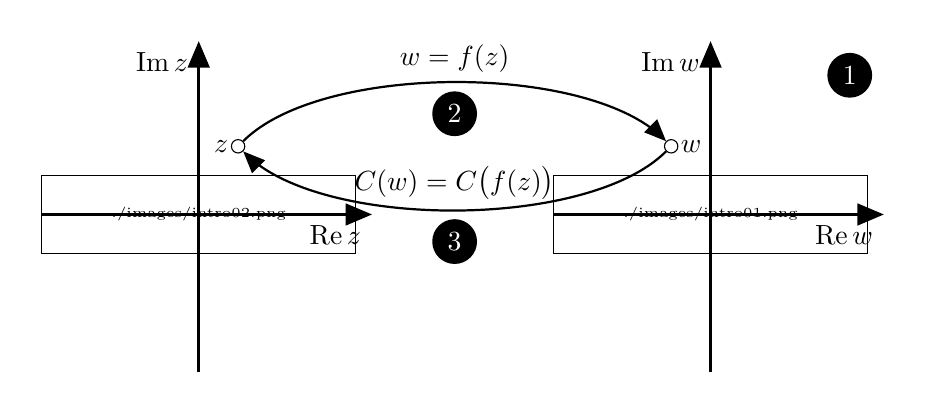
\begin{tikzpicture}[background rectangle/.style={fill=white}, show background rectangle,
                    istep/.style={color=white,fill=black,shape=circle,inner sep=1mm}]
  \path
    (0,0)coordinate(O) node[inner sep=0pt]{\pgfimage[width=4cm]{./images/intro02.png}}
    (6.5,0)coordinate(O2) node[inner sep=0pt]{\pgfimage[width=4cm]{./images/intro01.png}} ;
  \begin{scope}[very thick,-triangle 45]
    \draw (O) +(-2cm,0) -- ++(2.2cm,0) node[below left]{$\Re z$};
    \draw (O) +(0,-2cm) -- ++(0,2.2cm) node[below left]{$\Im z$};
    \draw (O2) +(-2cm,0) -- ++(2.2cm,0) node[below left]{$\Re w$};
    \draw (O2) +(0,-2cm) -- ++(0,2.2cm) node[below left]{$\Im w$};
  \end{scope}
  \draw (O) ++(60:1cm) node[inner sep=.6mm, shape=circle,draw](z){} node[left]{$z$};
  \draw (O2) ++(120:1cm) node[inner sep=.6mm, shape=circle,draw](w){} node[right]{$w$};
  \path (z) ++(45:1.5cm)coordinate(C1) (w) ++(135:1.5cm)coordinate(C2)
        (z) ++(-45:1.5cm)coordinate(C3) (w) ++(225:1.5cm)coordinate(C4);
  \begin{pgfinterruptboundingbox}
  \begin{scope}[thick, -triangle 45, every node/.style={pos=.5}]
    \draw (z) .. controls (C1) and (C2) .. (w) node[above]{$w=f(z)$} node[istep,below=1mm]{2};
    \draw (w) .. controls (C4) and (C3) .. (z) node[above]{$C(w)=C\bigl(f(z)\bigr)$} node[istep,below=1mm]{3};
    \path (O2) -- ++(45:5cm) node[istep]{1};
  \end{scope}
  \end{pgfinterruptboundingbox}
\end{tikzpicture}}
\end{document}
